%%%%%%%%%%%%%%%%%%%%%%%%%%%%%%%%%%%%%%%%%%%%%%%%%%%%%%%%%%%%%%%%%%%%%%
%   長野高専電子情報工学科 卒業論文テンプレート
%
%   Original by Takuma Yoshida, 2010
%   Modified by Shoichi Ito, 2014-
%
%%%%%%%%%%%%%%%%%%%%%%%%%%%%%%%%%%%%%%%%%%%%%%%%%%%%%%%%%%%%%%%%%%%%%%

% 卒業論文スタイルファイルの適用([a4,11pt]のようなオプションは不要)
\documentclass{eithesis}

% よくつかうパッケージの読み込み
\usepackage{verbatim}
\usepackage{itembkbx}
\usepackage{fancybox}
\usepackage{subcaption}
\usepackage{graphicx}
\usepackage{courier}
\usepackage{url}
\usepackage{fancyhdr}

\begin{document}
%%%%%%%%%%%%%%%%%%%%%%%%%%%%%%%%%%%%%%%%%%%%%%%%%%%%%%%%%%%%%%%%%%%%%%
%   表紙の設定
%%%%%%%%%%%%%%%%%%%%%%%%%%%%%%%%%%%%%%%%%%%%%%%%%%%%%%%%%%%%%%%%%%%%%%
\etGengou{令和2年度}      % 年度
\etTitle{RNNを用いたPOMDP環境での倒立振り子問題}     % 論文タイトル(日本語)
\etTitleEn{}    % 論文タイトル(英語)
\etDate{令和2年2月21日}   % 提出日(1月以降は年に注意)
\etAuthor{清水 翔仁}       % 著者フルネーム
\etLabName{西村研究室}     % 研究室名
\etMyProfessor{山根 智}    % 指導教員フルネーム
\etMakeTitle
%%%%%%%%%%%%%%%%%%%%%%%%%%%%%%%%%%%%%%%%%%%%%%%%%%%%%%%%%%%%%%%%%%%%%%
%   目次の出力
%%%%%%%%%%%%%%%%%%%%%%%%%%%%%%%%%%%%%%%%%%%%%%%%%%%%%%%%%%%%%%%%%%%%%%
% \pagenumbering{roman}
% \tableofcontents
% \clearpage
\pagenumbering{arabic}
%%%%%%%%%%%%%%%%%%%%%%%%%%%%%%%%%%%%%%%%%%%%%%%%%%%%%%%%%%%%%%%%%%%%%%
%   ヘッダー・フッターの設定
%%%%%%%%%%%%%%%%%%%%%%%%%%%%%%%%%%%%%%%%%%%%%%%%%%%%%%%%%%%%%%%%%%%%%%
\pagestyle{fancyplain}
\lhead{\leftmark}  % ヘッダー左側(\leftmarkのデフォルトはsectionhead)
\chead{}           % ヘッダー中央
\rhead{\rightmark} % ヘッダー右側(\rightmarkのデフォルトはchapterhead)
\lfoot{}           % フッター左側
\cfoot{\thepage}   % フッター中央(ページ番号)
\rfoot{}           % フッター右側

%%%%%%%%%%%%%%%%%%%%%%%%%%%%%%%%%%%%%%%%%%%%%%%%%%%%%%%%%%%%%%%%%%%%%%
%   論文本体
%%%%%%%%%%%%%%%%%%%%%%%%%%%%%%%%%%%%%%%%%%%%%%%%%%%%%%%%%%%%%%%%%%%%%%
\chapter{はじめに}
  % ここで,論文で採りあげていることについて,
  % 現状・問題意識・それが解決するとどんないいことがあるか
  % などについてデータを並べながら説明する.
  % 最後に,論文全体の構成(2章では○○について述べ,3章では・・・)を書く.
  % 全体で1〜2ページ.
  強化学習は,試行錯誤から学習する点で様々な問題に適用しやすいため,近年盛んに研究されている.DQN(Deep Q-Network) は,Q学習にディープラーニングを用いた強化学習のモデルで,ゲーム画面を入力したAtari 2600 の様々なゲームに対して人間より良い性能を実現した.しかし,DQN の入力はエージェントが観察した最近の4つのフレームのみを用いるため,意味がある行動をするために4ステップより昔の情報を必要とするような環境に対しては性能が低下する可能性がある.この欠点を解決するためにDRQN(Deep Recurrent Q-Network)が提案されている.DRQN は,DQNに循環神経網の一種であるLSTMを組み合わせることで過去の情報を扱う.さらにLSTMはより長期的な情報を考慮することで,現実で起こりうる不完全な情報にも対応できるため,POMDP(Partially Observable Markov Decision Process)の環境でより効果を発揮することができる.

  しかし,DRQNは学習の時にLSTMの初期状態をゼロベクトルで初期化するため,学習時に用いた情報のタイムステップより長い期間に対して学習することが難しいという欠点がある.そこで本研究では,LSTMの初期状態を与える方法を複数用意し,それぞれの実行結果についての考察を行う.
  % \clearpage

\chapter{原理}
  % 本章では,本研究で用いた手法の原理について説明する.
  \section{POMDP(Partially Observable Markov Decision Process)}
    状態遷移が確率的に生じる動的システムの確率モデルをMDPという.遷移する過程において,将来状態の条件付き確率分布が,現在状態のみに依存し,過去のいかなる状態にも依存しない.(マルコフ性)

    各時刻において過程 (process) はある状態 (state) を取り,意思を決定するエージェントはその状態において利用可能な行動 (action) を任意に選択する. その後過程はランダムに新しい状態へと遷移し,その際にエージェントは状態遷移に対応した報酬 (reward) を受けとる.よってMDPは以下の要素で構成される.
    \begin{equation}
    \begin{array}{l}\text { 行動集合 }: \mathcal{A}=\left\{a^{(1)}, a^{(2)}, \cdots,\right\} \\ \text { 状態集合 }: S=\left\{s^{(1)}, s^{(2)}, \cdots,\right\} \\ \text { 遷移関数 }: T_{i j k}=\operatorname{Pr}\left(s_{t+1}=s^{(j)} \mid s_{t}=s^{(i)}, a_{t}=a^{(k)}\right) \\ \text { 報酬関数 }: r = g(s, a) \\ \text { 初期状態確率 }: p_{0}=\operatorname{Pr}\left(s_{0}\right)\end{array}
    \end{equation}

    POMDPはエージェントの状態観測に不確実性を付加させることによりMDPを拡張したものである.

  \section{Q学習(Q-learning)}
    Q学習は強化学習における手法の一種である.Q学習はMDPにおいて全ての状態が十分にサンプリングできるようなエピソードを無限回試行した場合,最適な評価値に収束することがわかっている.Q学習では実行するルールに対しそのルールの有効性を示すQ値という値を持たせ,エージェントが行動するたびにその値を更新する.ここでいうルールとはある状態とその状態下においてエージェントが可能な行動を対にしたものである.例えばエージェントの現在の状態を$s_{t}$とし,この状態で可能な行動が$a$,$b$,$c$,$d$の4通りあるとする.このとき,エージェントは4つのQ値,$Q(s_{t},a)$,$Q(s_{t},b)$,$Q(s_{t},c)$,$Q(s_{t},d)$を元に行う行動を決定する.行動の決定方法は理論上では無限回数試行するならランダムでもQ値は収束するが,現実には収束を早めるため,なるべく Q値の大きな行動が高確率で選ばれるように行う.Q値の計算式を式(\ref{eq_Q})に示す.
    \begin{equation}\label{eq_Q}
      Q\left(s_{t}, a_{t}\right) = (1-\alpha) Q\left(s_{t}, a_{t}\right)+\alpha\left(r_{t+1}+\gamma \max _{a_{t+1}} Q\left(s_{t+1}, a_{t+1}\right)\right)
    \end{equation}
    ここで$\gamma$は割引率といい,将来の価値をどれだけ割り引いて考えるかのパラメータである.
  \section{DQN(Deep Q-Network)} \label{sec_dqn}
    Q値を最大化させる関数である最適行動価値関数を,ニューラルネットワーク(NN)を使った近似関数で求める手法.状態をNNの入力にし,出力層の各ノードが,各行動の行動価値を出力するようにする.

    強化学習において与えられるデータは時系列的に連続したものになっており,データ間に相関が出てしまうためバラバラにする必要がある.これをExperience Replayという.手法としては,まず一旦経験した状態/行動/報酬/遷移先をメモリーに蓄積し,学習を行う際はそこからランダムサンプリングして利用する.

  \section{RNN(Recurrent Neural Network)}
    RNNとは,Deep Learningの手法の一種であり,時系列データの分析に特化している.\figref{fig_RNN}に,RNNの模式図を示す.ここで,$x_t$を時刻$t$におけるRNNの入力,$h_t$を時刻$t$におけるRNNの出力とする.
    \begin{figure}[htbp]
      \centering
      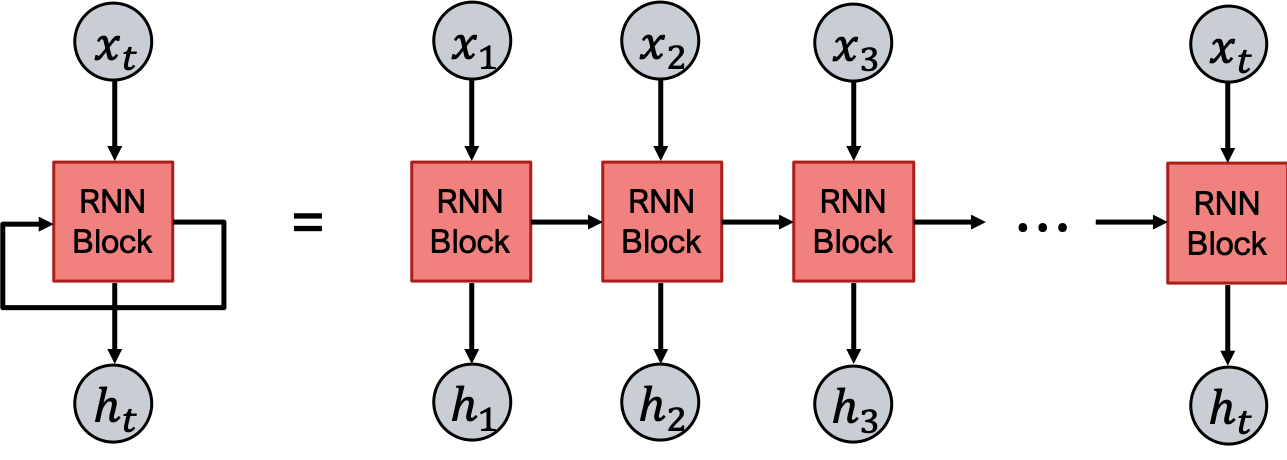
\includegraphics[width=14cm]{./images/RNN.png}
      \caption{展開されたRNN}
      \label{fig_RNN}
    \end{figure}

    \figref{fig_RNN}のように,RNNは内部にループ構造を持っている.これにより,前のステップでの分析結果を記憶し,データの時系列を理解することができる.しかし,RNNには長期依存性問題という欠点がある.長期依存性問題とは,記憶するステップ数が膨大になると計算が爆発するという問題である.そのため,現在単純なRNNはあまり使用されていない.

  \section{LSTM(Long Short Term Memory)}
    LSTMとは,RNNの長期依存性問題を解決した手法である.\figref{fig_RNN_inner}にRNNの内部を,\figref{fig_LSTM_inner}にLSTMの内部を示す.このとき,$\sigma$は0〜1を出力する関数,tanhは-1〜1を出力する関数とする.
    \begin{figure}[htbp]
      \centering
      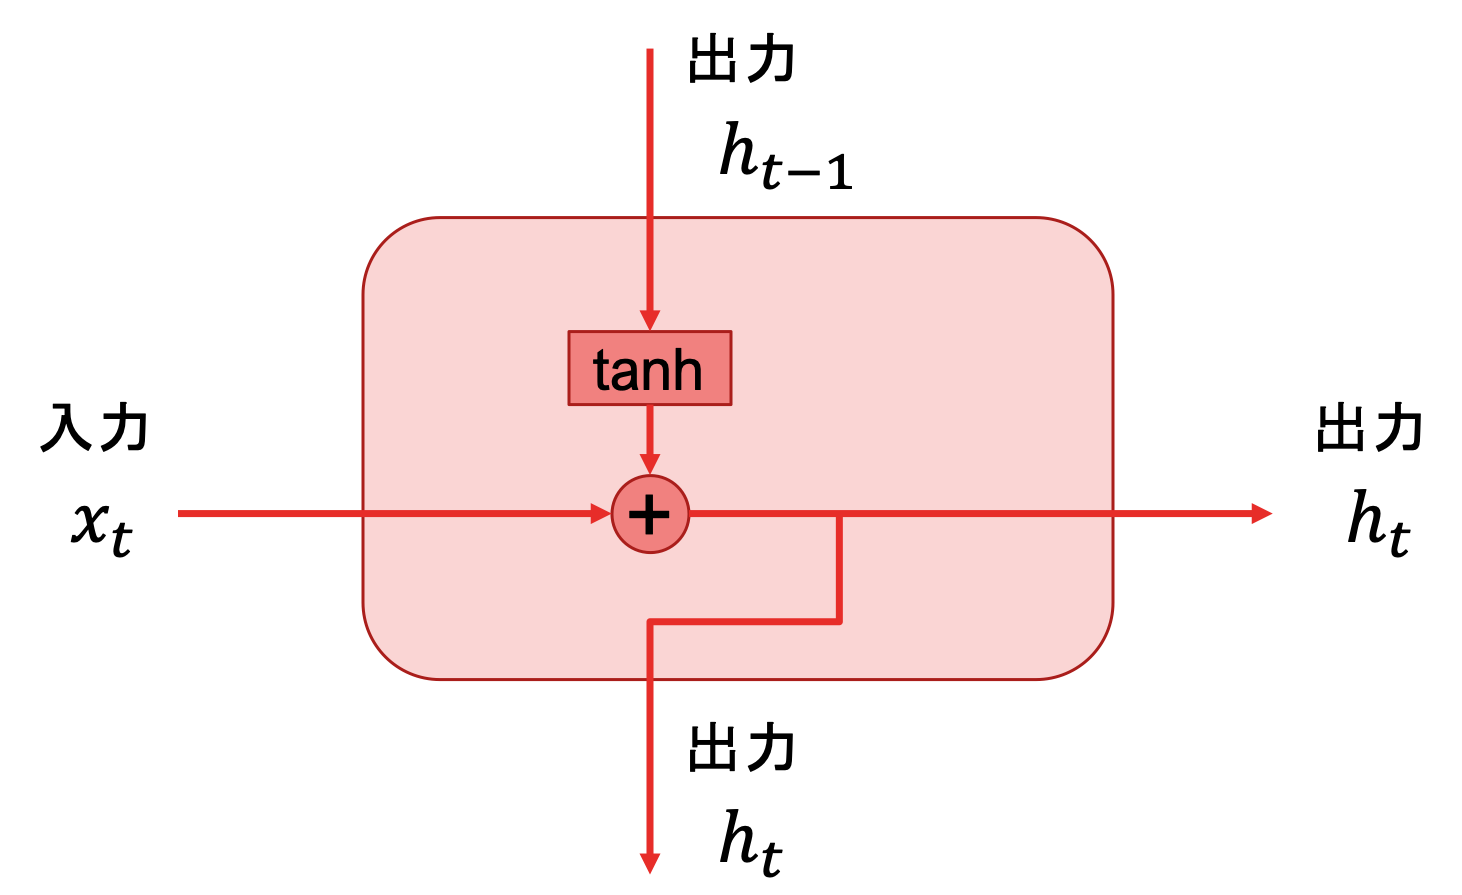
\includegraphics[width=14cm]{./images/RNN_inner.png}
      \caption{RNNの内部}
      \label{fig_RNN_inner}
    \end{figure}
    \begin{figure}[htbp]
      \centering
      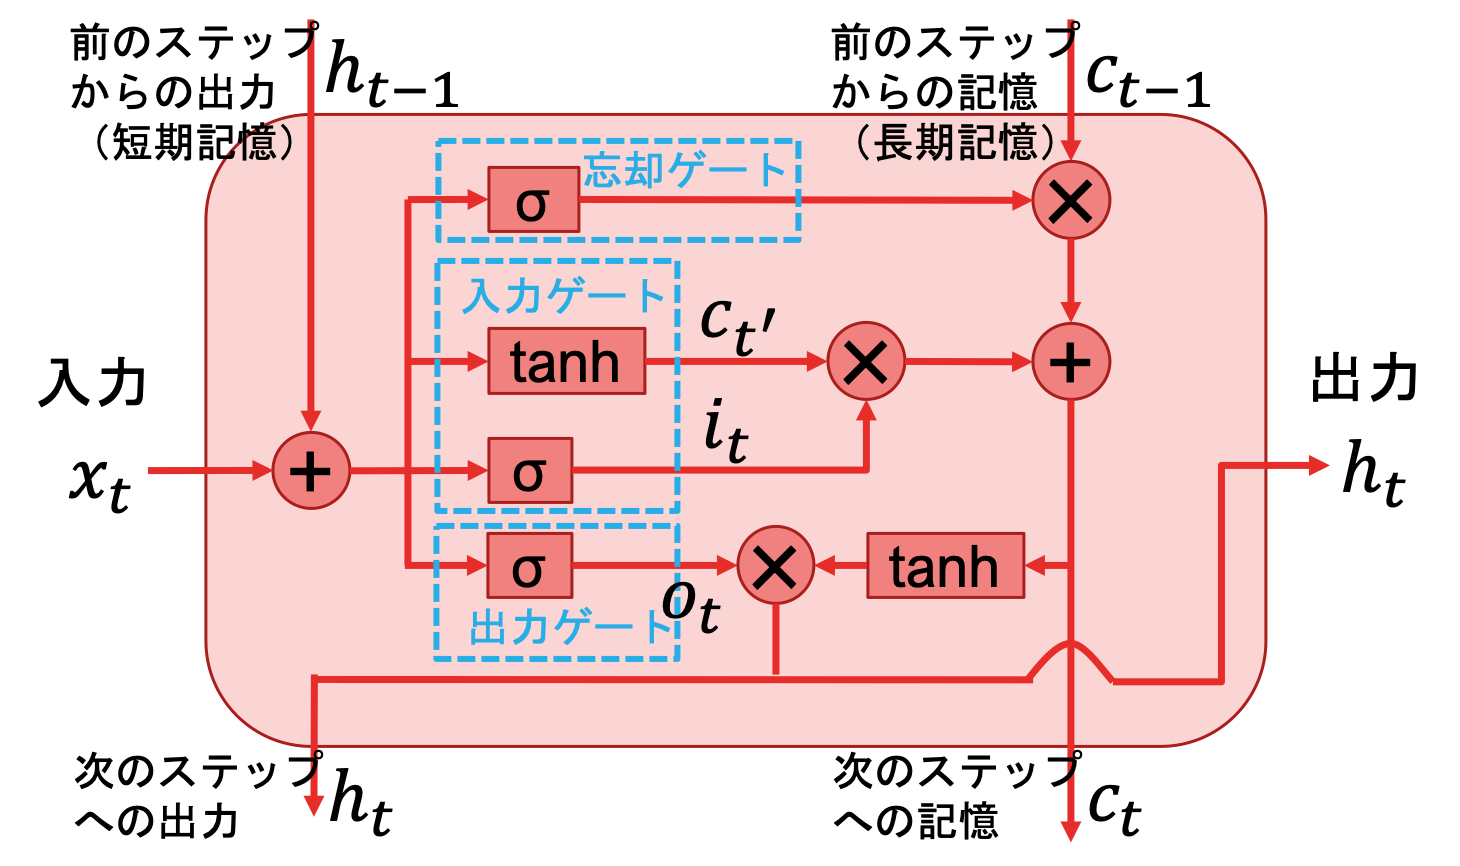
\includegraphics[width=14cm]{./images/LSTM_inner.png}
      \caption{LSTMの内部}
      \label{fig_LSTM_inner}
    \end{figure}

    \figref{fig_RNN_inner},\figref{fig_LSTM_inner}より,RNNは単一のtanh関数という非常に単純な構造に比べ,LSTMは4つの関数を含む複雑な構造をしている.

    ここで,\figref{fig_LSTM_inner}のLSTM内にデータが流れる手順について説明する.
    \begin{enumerate}
      \item 前のステップからの出力$h_{t-1}$と入力$x_t$が合流する.合流した信号はコピーされて4つのラインに分岐する.
      \item 一番上のラインの忘却ゲートでは,前のステップからの記憶一つ一つに対して,$\sigma$関数からの0〜1の値によって情報の取捨選択を行う.このとき1は情報を全て残し,0は全て捨てる.これにより,不要と思われる情報を捨てることで計算の爆発を防ぐ.
      \item 入力ゲートにおいて,前のステップからの出力$h_{t-1}$と入力$x_t$の合算を長期保存用に変換した上で,どの信号をどのくらいの重みで記憶に保存するか制御する.これは2つの手順で処理する.
        \begin{enumerate}
          \item tanh関数を用いて,入ってきた情報の情報量を削減し,必要な情報だけに変換された$c_{t'}$が出力する.
          \item $\sigma$関数の出力$i_t$によって,$h_{t-1}$を考慮して入力$x_t$の重みを調整する.
        \end{enumerate}
      \item 出力ゲートにおいて,上記の処理で取捨選択された長期記憶$c_t$の中で,短期記憶$h_t$に関する部分のみを出力する.これも2つの手順で処理する.
        \begin{enumerate}
          \item 前のステップからの記憶$c_{t-1}$と,入力$x_t$を変換した短期記憶$c_{t'}$を合算し,長期記憶$c_t$として出力する.これは,それぞれ既に忘却ゲートおよび入力ゲートで取捨選択が行われている.
          \item tanh関数に$c_t$を入力したものに対し,$\sigma$関数からの0〜1の値$o_t$によって情報の取捨選択を行う.
        \end{enumerate}
    \end{enumerate}

\chapter{実験方法}
  本章では,開発環境や実験方法について説明する.

  \section{開発環境}
    本研究ではGoogle Colaboratoryによって提供された開発環境を用いて実験を行なった.またColab内部で動作しているGPUはTesla T4である.

  \section{実験方法}\label{sec_program}
    今回,LSTMの初期状態を与える方法を検証するため,DQN,DRQN,DRQN-Stack,DRQN-Store-State,R2D2の5つの手法を用いて実装されたプログラムをそれぞれ用意した.それぞれのプログラムの概要について説明を行う.
    \subsection{DQN}
      第\ref{sec_dqn}章において説明したDQNを用いたプログラム.このプログラムではLSTMは使用していない.
    \subsection{DRQN}
      DRQNを用いたプログラム.DRQNとはDQNにLSTMを組み込んだ手法.時系列表現を獲得することでPOMDPに対応でき,過去の情報を使って解くタスクに強い.

      このプログラムではエピソードからランダムに軌跡を取り出し,LSTMの初期状態をzero入力して学習を行う.これをBootstrapped Random Updatesという.シンプルかつランダムにサンプリングできるメリットはあるが,初期状態をzero入力するためLSTMが適切な表現を獲得できない可能性がある.
      Bootstrapped Random Updatesの模式図を図\ref{fig_random}に示す.
      \begin{figure}[htbp]
        \centering
        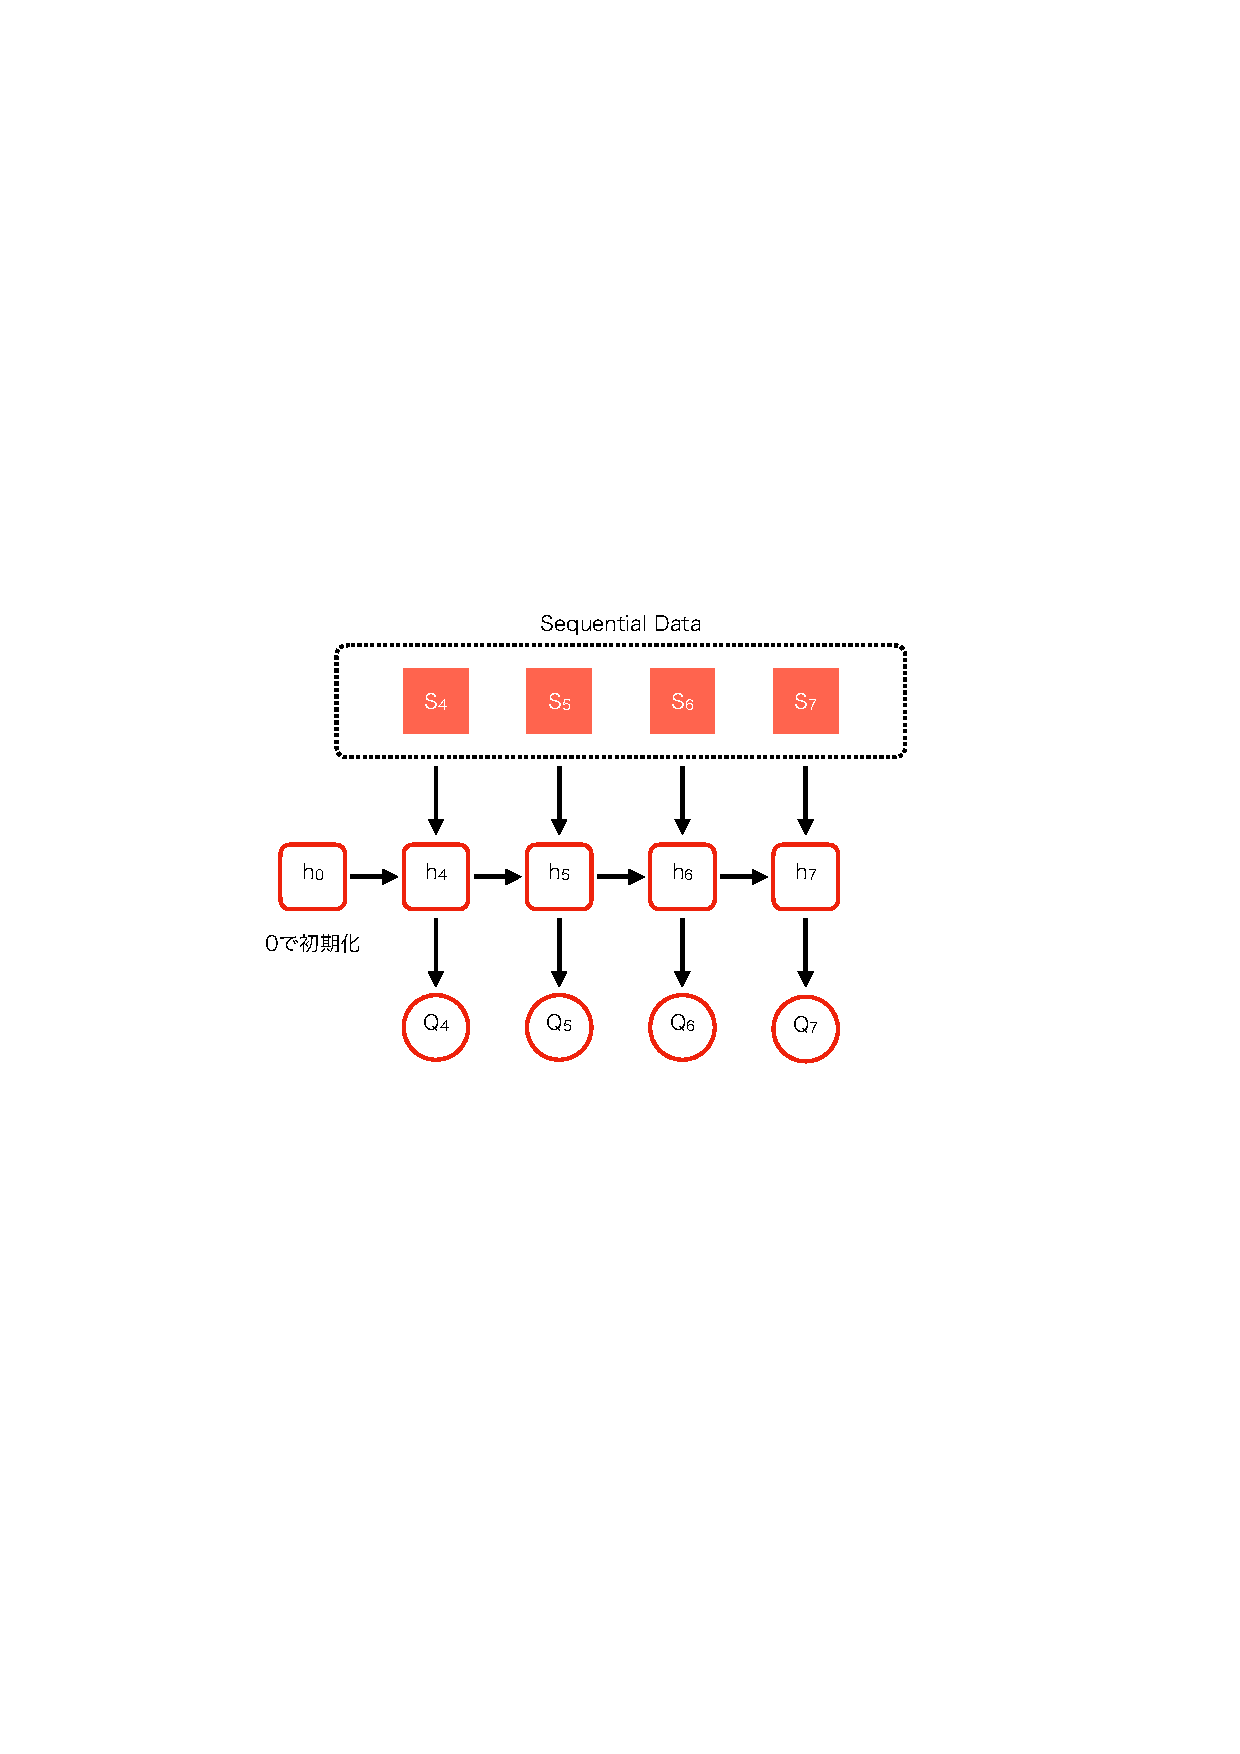
\includegraphics[width=12cm]{./images/random.pdf}
        \caption{Bootstrapped Random Updates}
        \label{fig_random}
      \end{figure}
    \subsection{DRQN-Stack}
      DRQNを用いたプログラム.このプログラムでは1エピソード全部のデータを使って学習を行う.これをBootstrapped Sequential Updatesという.LSTM初期化で困ることはないが,バリアンスが大きい,エピソード長が可変などの問題がある.Bootstrapped Sequential Updatesの模式図を図\ref{fig_sequential}に示す.
      \begin{figure}[htbp]
        \centering
        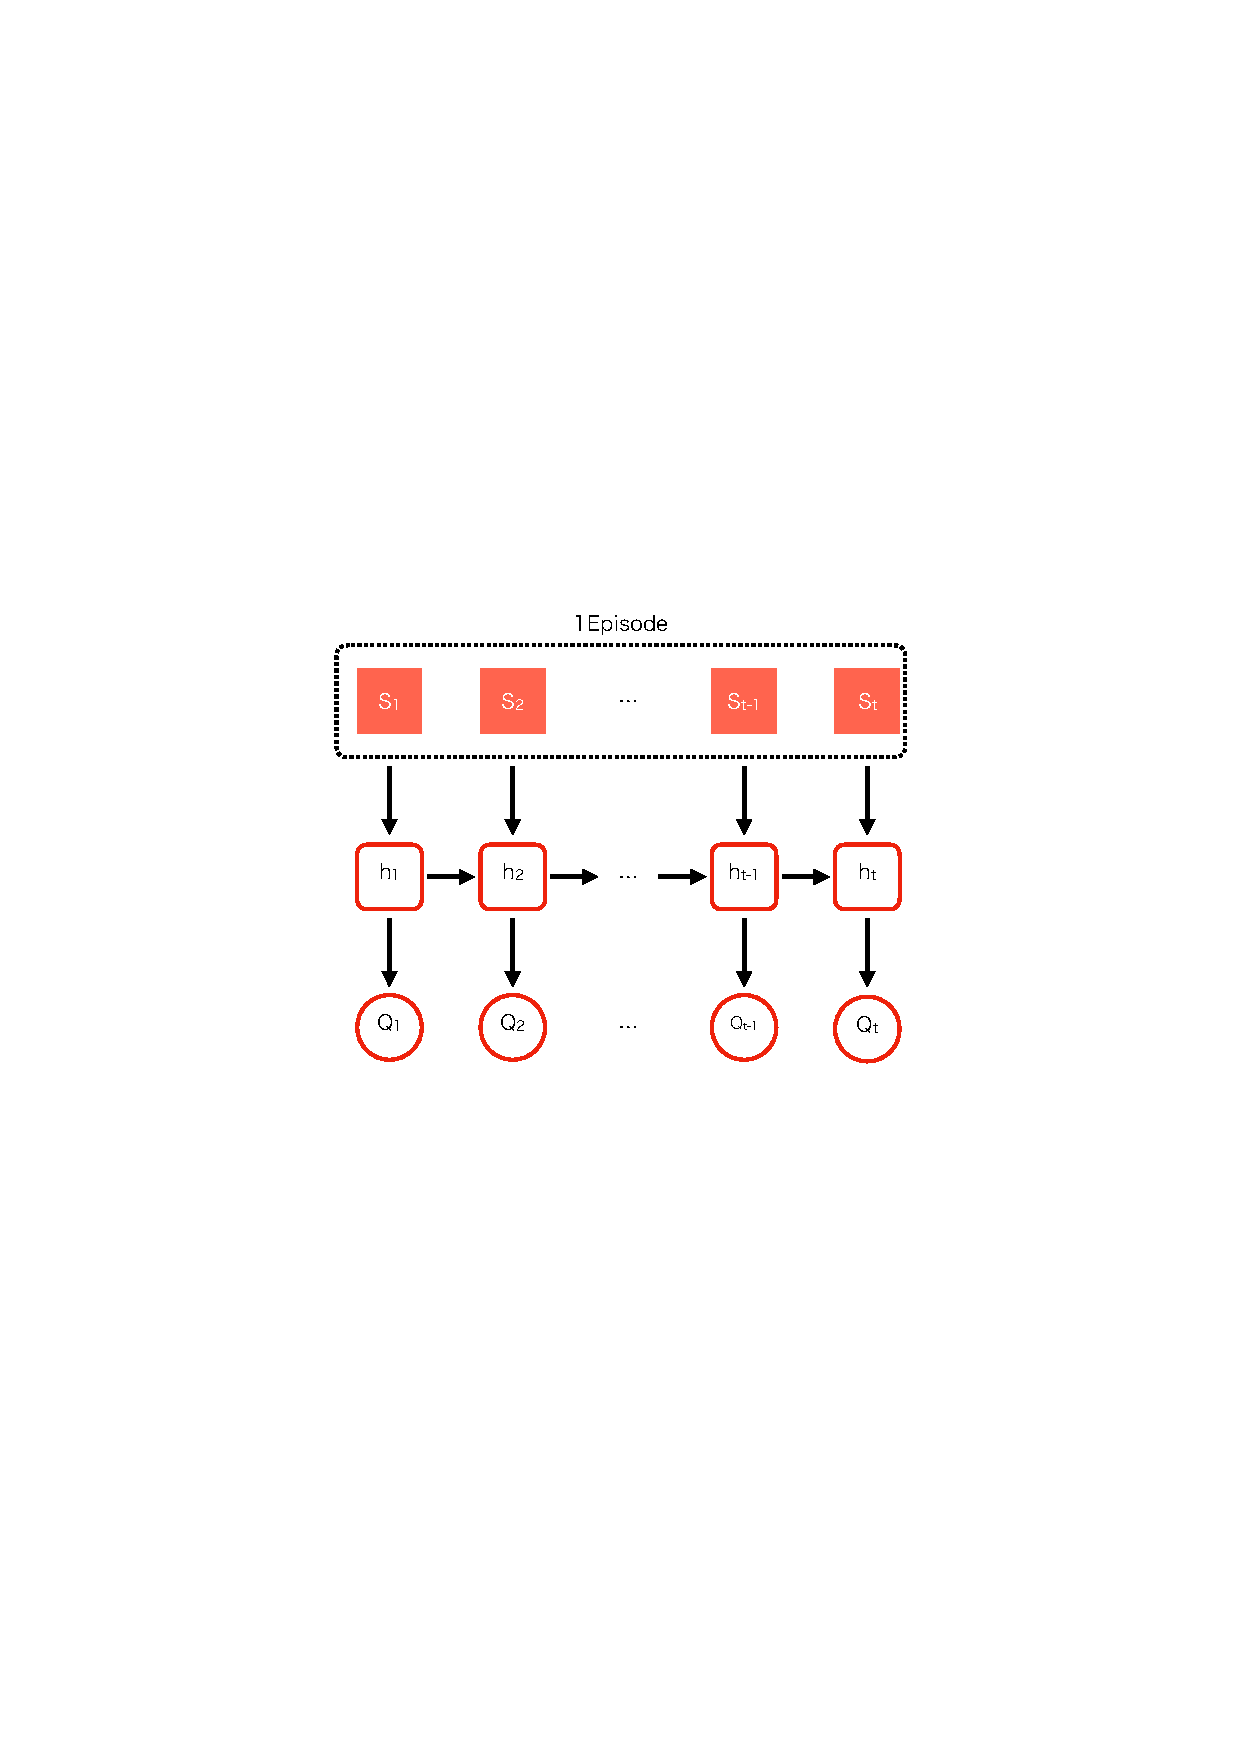
\includegraphics[width=10cm]{./images/sequential.pdf}
        \caption{Bootstrapped Sequential Updates}
        \label{fig_sequential}
      \end{figure}
    \subsection{DRQN-Store-State}\label{sec_ss}
      DRQNを用いたプログラム.このプログラムではBootstrapped Random Updatesに加えて,Replay Bufferに経験$e!$とともにその時のLSTMのhidden stateを貯めておく.これによりLSTMの初期状態問題を改善している.模式図を図\ref{fig_storedState}に示す.
      \begin{figure}[htbp]
        \centering
        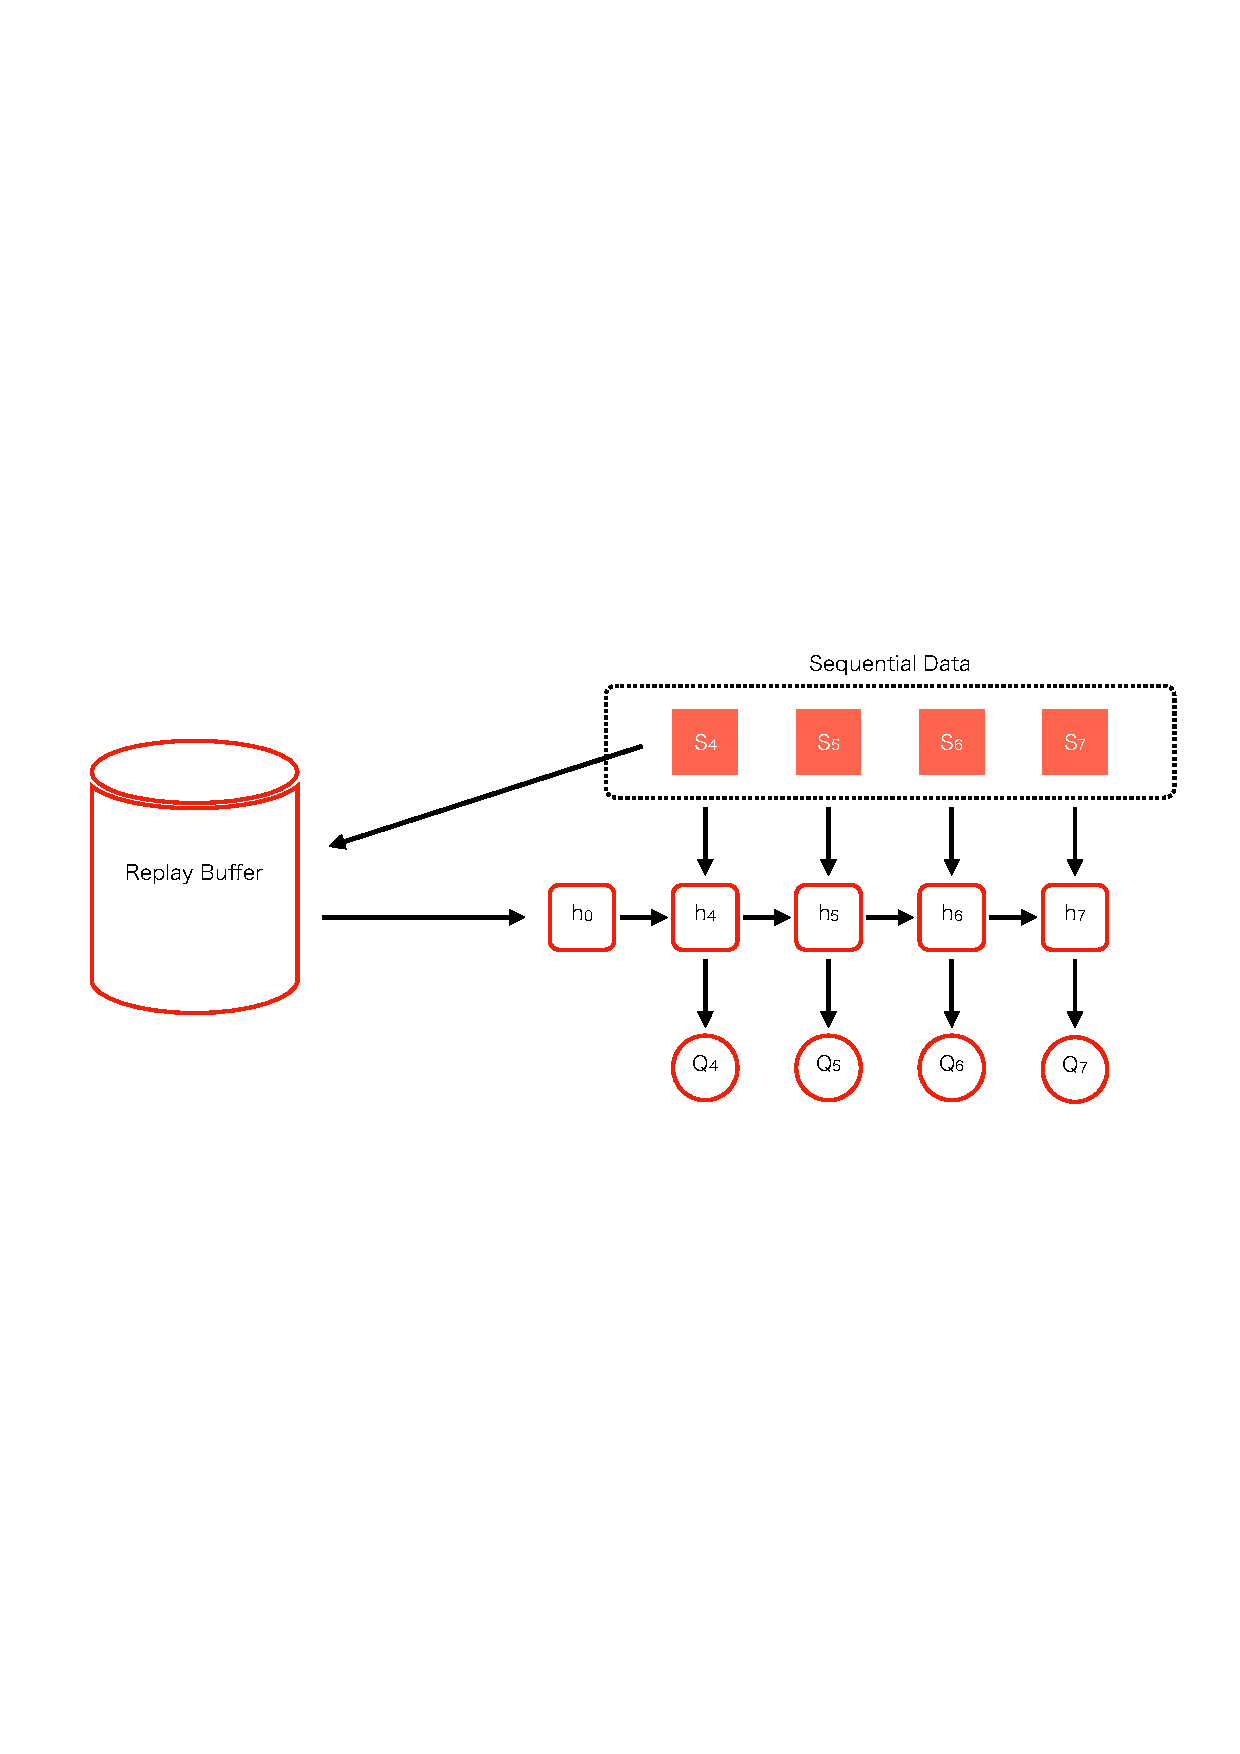
\includegraphics[width=12cm]{./images/storedState.pdf}
        \caption{Bootstrapped Random Updates + Replay Buffer}
        \label{fig_storedState}
      \end{figure}
    \subsection{R2D2}
      DRQNを用いたプログラム.このプログラムでは第\ref{sec_ss}節で述べたBootstrapped Random UpdatesとReplay Bufferの組み合わせに加えて,Burn-inという手法を採用している.これは最初は学習を行わずデータだけを流し今のネットワークの重みに慣れさせるという手法である.これにより正確なhidden stateを復元することができる.模式図を図\ref{fig_burnIn}に示す.
      \begin{figure}[htbp]
        \centering
        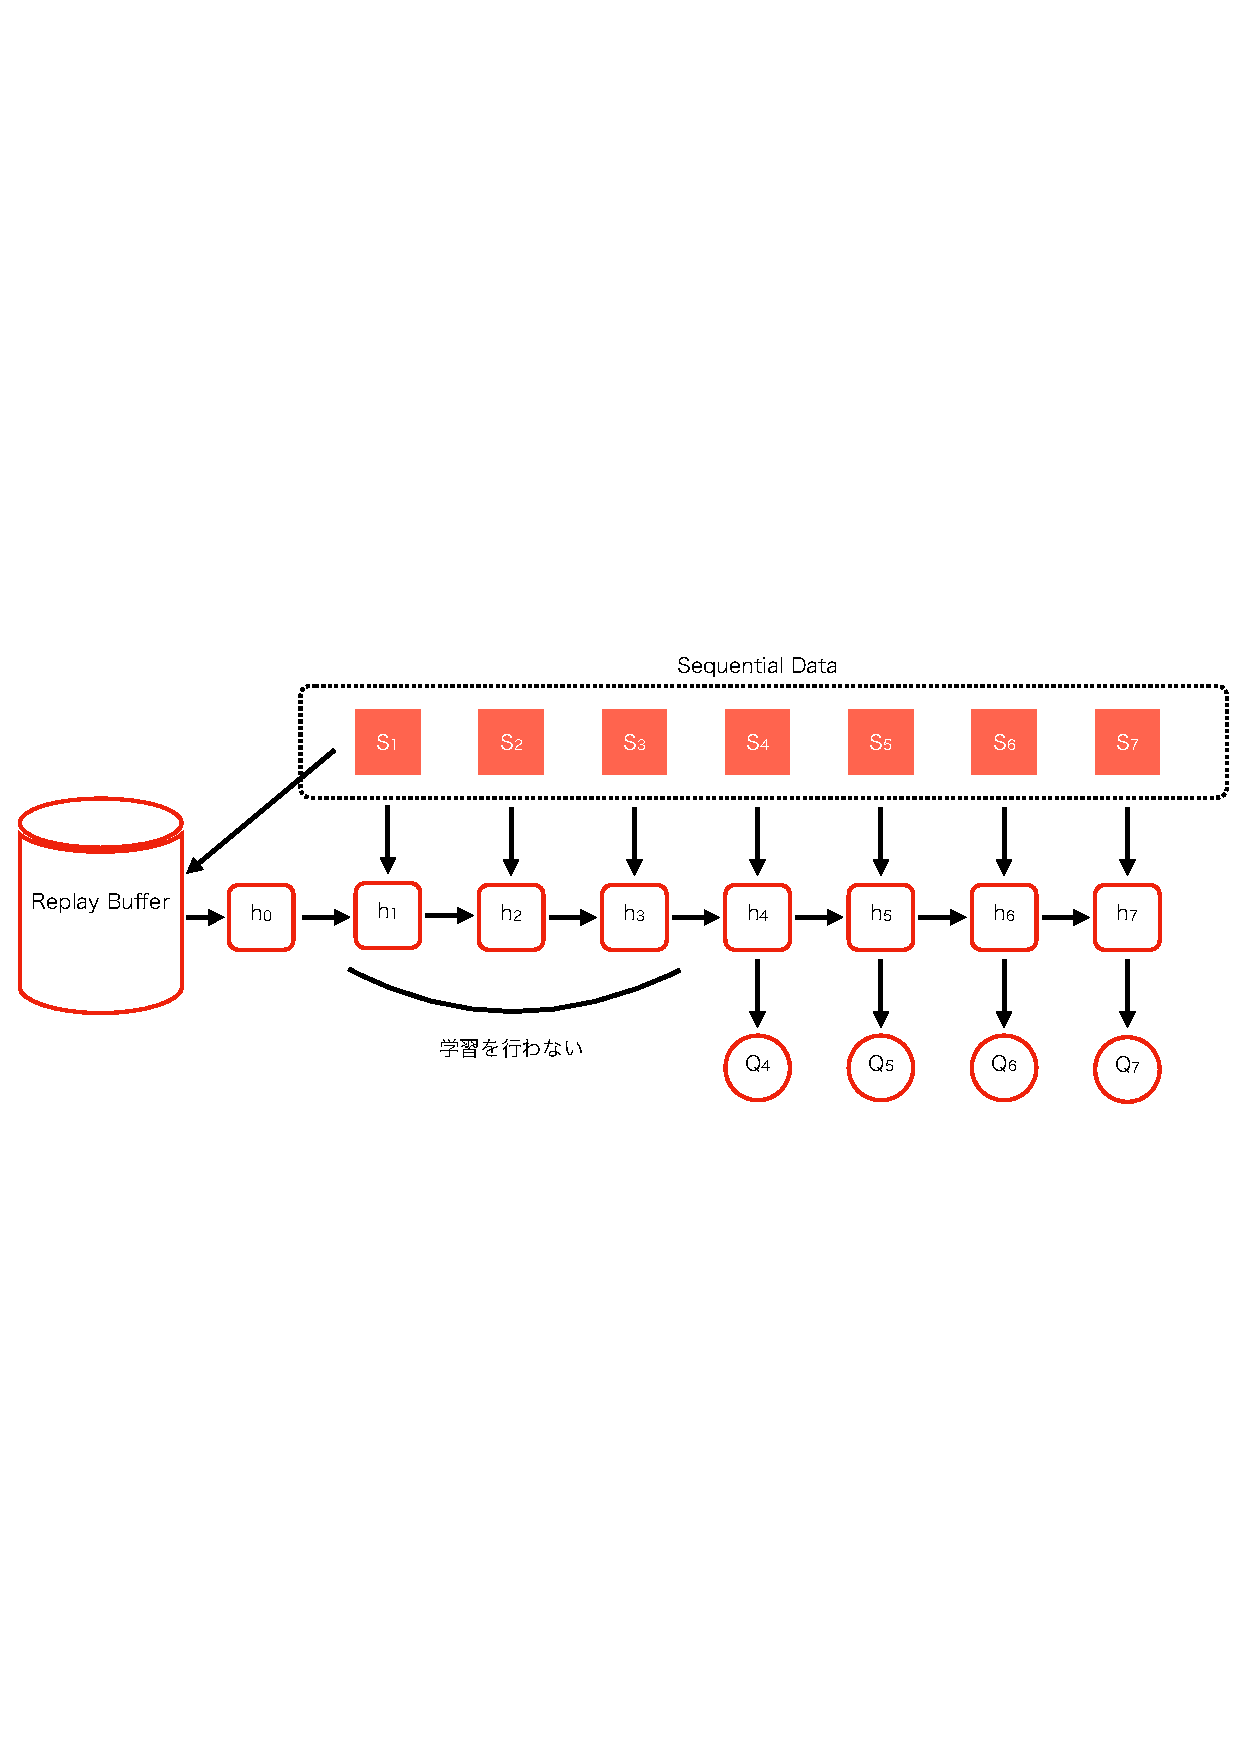
\includegraphics[width=12cm]{./images/burnIn.pdf}
        \caption{Bootstrapped Random Updates + Replay Buffer + Burn-in}
        \label{fig_burnIn}
      \end{figure}

\chapter{結果}
  第\ref{sec_program}章で述べた5つのプログラムの実行結果を示す.

  DQNの実行結果を以下に示す.これより,scoreは伸びず収束しないまま終了していることがわかる.
  \begin{breakitembox}[l]{DQNの実行結果}
    \begin{verbatim}
0 episode | score: 30.00 | epsilon: 1.00
10 episode | score: 29.53 | epsilon: 1.00
20 episode | score: 28.56 | epsilon: 1.00
30 episode | score: 28.49 | epsilon: 1.00
40 episode | score: 27.54 | epsilon: 1.00
                  ...
29950 episode | score: 20.64 | epsilon: 0.10
29960 episode | score: 20.01 | epsilon: 0.10
29970 episode | score: 19.50 | epsilon: 0.10
29980 episode | score: 19.06 | epsilon: 0.10
29990 episode | score: 19.01 | epsilon: 0.10
    \end{verbatim}
  \end{breakitembox}

  DRQNの実行結果を以下に示す.これより,DQNと同様にscoreは伸びず収束しないまま終了していることがわかる.これは初期状態がzero入力されたことによるものだと考えられる.
  \begin{breakitembox}[l]{DRQNの実行結果}
    \begin{verbatim}
0 episode | score: 26.00 | epsilon: 1.00
10 episode | score: 25.24 | epsilon: 1.00
20 episode | score: 24.43 | epsilon: 1.00
30 episode | score: 23.89 | epsilon: 1.00
40 episode | score: 23.61 | epsilon: 1.00
                  ...
29950 episode | score: 18.53 | epsilon: 0.10
29960 episode | score: 19.06 | epsilon: 0.10
29970 episode | score: 18.99 | epsilon: 0.10
29980 episode | score: 19.30 | epsilon: 0.10
29990 episode | score: 19.10 | epsilon: 0.10
    \end{verbatim}
  \end{breakitembox}

  DRQN-Stackの実行結果を以下に示す.これより,DQNやDRQNとは違いscoreが200近くで収束していることがわかる.これはBootstrapped Sequential Updatesによって初期状態が与えられたことによるものだと考えられる.
  \begin{breakitembox}[l]{DRQN-Stackの実行結果}
    \begin{verbatim}
0 episode | score: 26.00 | epsilon: 1.00
10 episode | score: 25.50 | epsilon: 1.00
20 episode | score: 26.68 | epsilon: 1.00
30 episode | score: 26.13 | epsilon: 1.00
40 episode | score: 25.58 | epsilon: 1.00
                  ...
700 episode | score: 162.81 | epsilon: 0.10
710 episode | score: 170.72 | epsilon: 0.10
720 episode | score: 180.14 | epsilon: 0.10
730 episode | score: 191.17 | epsilon: 0.10
740 episode | score: 199.45 | epsilon: 0.10
    \end{verbatim}
  \end{breakitembox}

  DRQN-Store-Stateの実行結果を以下に示す.これより,DRQN-Stackに比べ,収束までのステップ数が長いことがわかる.
  \begin{breakitembox}[l]{DRQN-Stackの実行結果}
    \begin{verbatim}
0 episode | score: 23.00 | epsilon: 1.00
10 episode | score: 22.77 | epsilon: 1.00
20 episode | score: 22.79 | epsilon: 1.00
30 episode | score: 22.82 | epsilon: 1.00
40 episode | score: 22.67 | epsilon: 1.00
                  ...
820 episode | score: 148.15 | epsilon: 0.10
830 episode | score: 147.86 | epsilon: 0.10
840 episode | score: 158.67 | epsilon: 0.10
850 episode | score: 169.52 | epsilon: 0.10
860 episode | score: 192.27 | epsilon: 0.10
    \end{verbatim}
  \end{breakitembox}

  R2D2の実行結果を以下に示す.これより,他のプログラムに比べ最も短いステップ数で収束していることがわかる.これはBurn-inによってhidden stateの復元期間を設けることでより正確な学習ができていると考えられる.
  \begin{breakitembox}[l]{DRQN-Stackの実行結果}
    \begin{verbatim}
0 episode | score: 10.00 | epsilon: 1.00
10 episode | score: 11.90 | epsilon: 1.00
20 episode | score: 12.74 | epsilon: 1.00
30 episode | score: 14.22 | epsilon: 1.00
40 episode | score: 15.35 | epsilon: 1.00
                  ...
490 episode | score: 140.98 | epsilon: 0.10
500 episode | score: 159.77 | epsilon: 0.10
510 episode | score: 179.90 | epsilon: 0.10
520 episode | score: 192.32 | epsilon: 0.10
530 episode | score: 200.57 | epsilon: 0.10
    \end{verbatim}
  \end{breakitembox}

\chapter{まとめ}
  % 「はじめに」で振った話や問題意識がどれだけ回収できているか,
  % なにが問題として残ったのか.
  % あらためて研究のはじめから終わりまでの全体を俯瞰してのまとめを書く.
  % どうせやる予定のない「今後の予定」は書いてはいけない.
  本研究の目標である,LSTMの初期状態問題の検証を行うことができた.
  また今回使用した5つのプログラムの内3つのプログラムでは,結果が収束したため初期状態問題は改善されていると考えられる.
  特にR2-D2においては他のプログラムに比べ200ステップ数ほど早い段階で収束しており,Bootstrapped RandomUpdatesとReplay Buffer,Burn-inの組み合わせがうまく機能していると考えられる.

%%%%%%%%%%%%%%%%%%%%%%%%%%%%%%%%%%%%%%%%%%%%%%%%%%%%%%%%%%%%%%%%%%%%%%
%   謝辞と参考文献
%%%%%%%%%%%%%%%%%%%%%%%%%%%%%%%%%%%%%%%%%%%%%%%%%%%%%%%%%%%%%%%%%%%%%%
% \chapter*{謝辞}
% 	% ここは自由に書いて良い.その人の協力なくしてこの研究は成し遂げられなかった
% 	% と思われる人への謝意をあらわす.名前は基本的にフルネームで入れる.
% 	本研究を進めるに当たり,西村治教授から多大な助言を賜りました.厚く感謝を申し上げます.また一年間同じ研究室で研究を行ってきた青沼葵さん,櫻井優太さん,関谷賢二さん,山本七海さんにも感謝の意を表します.
% 	\begin{flushright}
% 		2020年2月

% 		清水翔仁
% 	\end{flushright}

% \begin{thebibliography}{99}
% \bibitem{rinri}{鬼頭 葉子: 技術者の倫理, ナカニシヤ出版, 2018.}
% \bibitem{kishow}{気象庁 | 数値予報課報告・別冊第64号(令和2年2月16日現在): \url{https://www.jma.go.jp/jma/kishou/books/nwpreport/64/chapter1.pdf}}
% \bibitem{data}{気象庁 | 過去の気象データ・ダウンロード(令和2年2月16日現在): \url{https://www.data.jma.go.jp/gmd/risk/obsdl/index.php}}
% \bibitem{oreilly}{Antonio Gulli・Sujit Pal(著),大串正矢・久保隆宏・中山光樹(訳): 直感Deep Learning, 株式会社オライリー・ジャパン, 2019.}
% \bibitem{python}{Sebastian Raschka・Vahid Mirjalili(著),株式会社クイープ(訳): [第2版]Python機械学習プログラミング, 株式会社インプレス, 2018.}
% \bibitem{tb}{TensorBoard(令和2年1月20日現在): \url{https://www.tensorflow.org/tensorboard}}
% \end{thebibliography}

\end{document}
